\documentclass[12pt,a4paper]{article}

\usepackage[utf8]{inputenc}
\usepackage[MeX]{polski}
\usepackage{graphicx}   %do rysunków
\usepackage{wrapfig}    %do rysunków otoczonych tekstem
\usepackage{color}      %do użycia podst. kolorów oraz zdefiniowanych kolorów 
\usepackage{float}
\usepackage{url}
\usepackage{amsmath}
\usepackage[strings]{underscore}
\usepackage[center]{caption}
%do kolorowych referencji do rysunków, cytowań:
\usepackage{multicol}
\usepackage{colortbl}
%\usepackage[colorlinks=true,linkcolor=firebrick,citecolor=green]{hyperref}
\renewcommand{\refname}{Źródła}
\textwidth=16cm
\textheight=23cm
\topmargin=-2cm
\oddsidemargin=0cm


\title{Wstęp do fizyki ciała stałego - projekt}
\author{Jan Biały}
\date{Styczeń 2024}
%%%%%%%%%%%%%%%%%%%%%%%%%%%%%%%%%%%%%%%%%%%%%%%%%%%%%
\begin{document}
\maketitle

\begin{table}[h!]
\centering
\begin{tabular}{|p{2.1cm}|p{2.1cm}|p{2.1cm}|p{2.1cm}|p{2.1cm}|p{2.1cm}|}\hline
\multicolumn{2}{|c|}{\textbf{Wstęp do fizyki ciała stałego}}
& \multicolumn{4}{c|}{\textbf{Projekt 1, zestaw 5}} \\ \hline
\multicolumn{2}{|l|}{(Jan Biały)} & e-mail: & \multicolumn{3}{c|}{01169730@pw.edu.pl} \\ \hline
data:  & 11.01.2024 & nr indeksu: & 323614 & grupa: & Z1 \\ \hline
\multicolumn{6}{|c|}{\begin{tabular}[c]{@{}c@{}}Oświadczam, że jestem jedynym autorem/jedyną
autorką niniejszego projektu.\\Jestem świadomy/świadoma odpowiedzialności w przypadku podania
fałszywej informacji.\\ \\ (podpis studenta)\end{tabular}} \\ \hline
\end{tabular}
\end{table}
\clearpage
\section*{Cel projektu}
Celem projektu było utrwalenie wiedzy nabytej na ćwiczeniach oraz wykładach z przedmiotu Wstęp do fizyki ciała stałego. Ten dokument jest sprawozdaniem z wykonania zadań projektowych zadanych przez prowadzącego przedmiot. 
\section*{Zadanie 1}
W tym zadaniu należało wykreślić zależność odległości między jądrami atomowymi od potencjału pewnego wiązania chemicznego na podstawie danych numerycznych zawartych w pliku \textit{zad1_wch_n.txt} oraz przeanalizowanie tych danych w celu wyznaczenia:
\begin{itemize}
\item równowagową długość wiązania $r0$ w $[\AA]$,
\item wartość energii wiązania $U(r_0)$ w $[eV]$,
\item stałą siłową wiązania $k$ w $[\frac{N}{m}]$,
\item współczynnik anharmoniczności $\gamma$ w $[\frac{N}{m^2}]$
\end{itemize}
Do wyznaczenia powyższych danych należało dopasować odpowiedni wielomian do wykresu danych numerycznych z analizowanego pliku.
\begin{figure}[H]
\centering
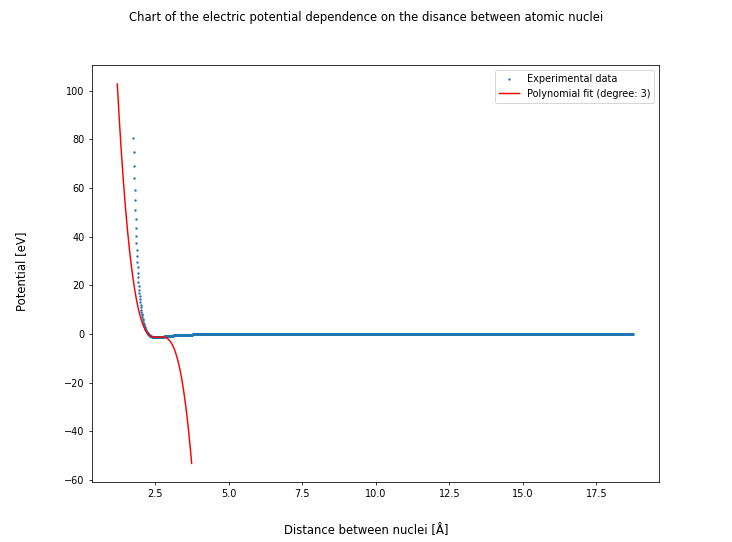
\includegraphics[scale=0.65]{D:/My Files/Python/DataPyTool/plots/zad1.png}
\vspace{-0,2cm}
\label{Wykres zależności potencjału analizowanego wiązania chemicznego od odległości między jądrami atomowymi.}
\caption{Wykres zależności potencjału analizowanego wiązania chemicznego od odległości między jądrami atomowymi.}
\end{figure}
Minimum tej zależności przypadało na punkt $(2,52;9131898489)$. Wartość współrzędnej $x$ tego punktu oznacza wartość równowagowej długości wiązania $r0$  zaś współrzędna $y$ tego punktu jest wartością energii wiązania $U(r_0)$ zatem.
\begin{itemize}
\item $r0 = 2,52 [\AA]$
\item $U(r_0) = -1,31898489 [eV]$
\end{itemize}
\begin{figure}[H]
\centering
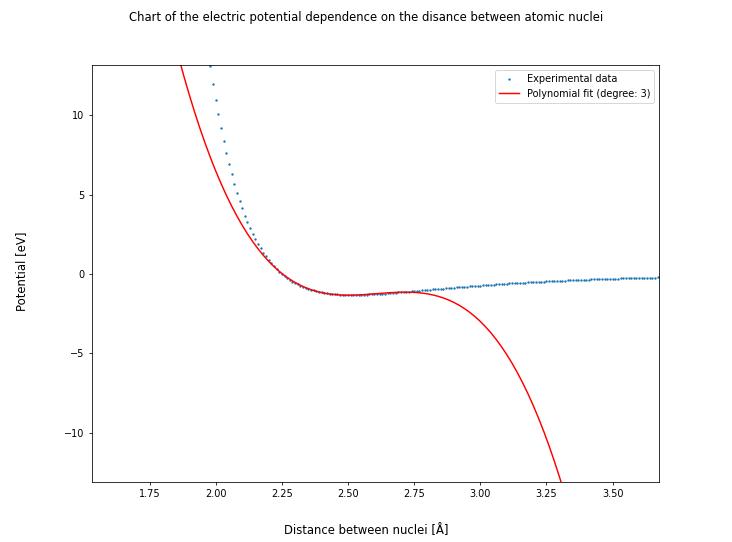
\includegraphics[scale=0.65]{D:/My Files/Python/DataPyTool/plots/zad1closeup.png}
\vspace{-0,2cm}
\label{Wykres zależności potencjału analizowanego wiązania chemicznego od odległości między jądrami atomowymi (zbliżenie na dopasowanie wielomianu do wykresu).}
\caption{Wykres zależności potencjału analizowanego wiązania chemicznego od odległości między jądrami atomowymi(zbliżenie na dopasowanie wielomianu do wykresu).}
\end{figure}
Generacja jak i dopasowanie wielomianu odbyło się przy użyciu programu DataPyTool własnego autorstwa. Do wykresu danych dopasowano wielomian trzeciego stopnia o ogólnym wzorze $ax^3+bx^2+cx+d$. Wielomian dopasowano na przedziale od 45 do 150 numeru pomiaru czyli na przedziale (2,2;2,55) odległości między jądrami atomowymi.
\\
Dopasowany do danych wielomian miał postaci:
\begin{equation}
-37,85x^3+296,24x^2-771,46x+665,95
\end{equation}
Wartości współczynników przy potęgach $x^3$ jak i $x^3$ wykorzystano do obliczenia stałej siłowej $k$ oraz współczynnika anharmoniczności $\gamma$, ponieważ zależność $U(r)$ można rozwinąć w szereg Taylor'a wokół analizowanego otoczenia. 
Zatem wartość stałej siłowej wynosi:
\begin{equation}
k=2!\cdot b = 2!\cdot 296,24 = 592,48\frac{eV}{\AA^2} = 9492,576121 \frac{N}{m},
\end{equation}
zaś współczynni anharmoniczności wynosi:
\begin{equation}
\gamma = 3!\cdot a = 3! \cdot 37,85 = 227,1 \frac{eV}{\AA^3} = 3,638543136\cdot 10^{13} \frac{N}{m^2}
\end{equation}
\section*{Zadanie 2}
W tym zadaniu należało przeanalizować dane z pliku \textit{zad2_bat_5.txt} opisujące proces rozładowania ogniwa litowego z katodą z krystalizowanego szkła $90V_2O_5\cdot10B_2O_3$ oraz wyznaczenie na podstawie tych danych wartości:
\begin{itemize}
\item teoretycznej pojemności grawimetrycznej $Q_t$ ogniwa,
\item doświadczalnej pojemności grawimetrycznej $Q_d$ ogniwa,
\item stosunku teoretycznej pojemności grawimetrycznej do pojemności doświadczalnej
\item napięcie nominalne ogniwa $U_{nom}$. 
\end{itemize}
Dla zestawu 5 podane były masa materiału aktywnego $m=2,06[mg]$ oraz natężenie prądu $I,162,74[\mu A]$.
\\
Wartość teoretycznej pojemności grawimetrycznej wyznaczono z zależności:
\begin{equation}
Q_t = \frac{neN_A}{M_{V_2O_5}} = 3\cdot 529,23[\frac{C}{g}] = 441[\frac{mAh}{g}],
\end{equation}
gdzie $e=1,602176634 \cdot 10^{-19}[C]$ - ładunek elementarny, $N_A = 10{-10}$ - stała Avogadro, $M_{V_2O_5} = 2\cdot 51[\frac{g}{mol}] + 5\cdot 16 [\frac{g}{mol}] = 182[\frac{g}{mol}]$ - masa molowa $V_2O_5$ biorącego udział w interkalacji, $n = 3$ - liczba interkalowanych jonów litu na jeden jon $V_2O_5$. 
\begin{figure}[H]
\centering
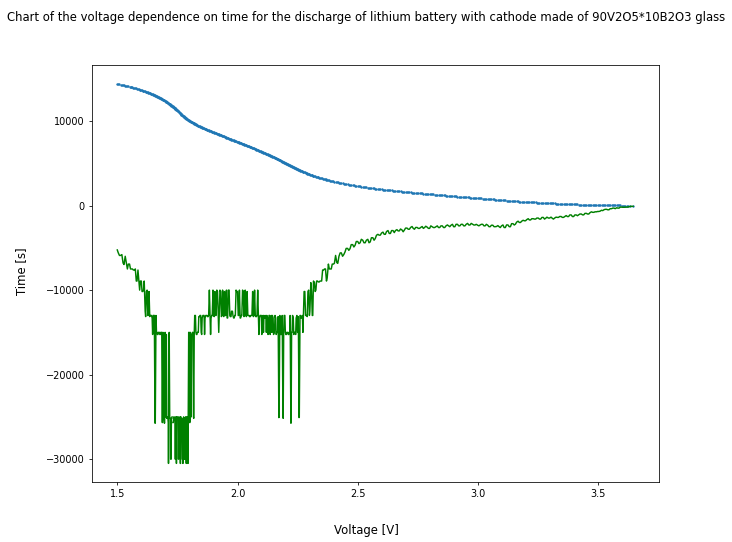
\includegraphics[scale=0.65]{D:/My Files/Python/DataPyTool/plots/zad2.png}
\vspace{-0,2cm}
\label{Wykres zależności napięcia badanym ogniwie w zależności od czasu dla procesu rozładowania wraz numerycznie policzoną pochodną wykresu.}
\caption{Wykres zależności napięcia badanym ogniwie w zależności od czasu dla procesu rozładowania wraz numerycznie policzoną pochodną wykresu.}
\end{figure}
Na podstawie podanych danych wyznaczono doświadczalną pojemność grawimetryczną $Q_d$ ze wzoru:
\begin{equation}
Q_d = \frac{\int\limits_0^T U(t)}{T} = 
\end{equation}
gdzie $T$
\vspace{2cm}
\noindent


\end{document}